\documentclass[tikz,border=5pt]{standalone}
\usepackage{amsmath,amssymb}
\usetikzlibrary{decorations.pathreplacing,calc}

\definecolor{accent}{RGB}{0, 100, 170}
\definecolor{highlight}{RGB}{200, 60, 30}
\definecolor{darkgreen}{RGB}{0, 120, 60}
\definecolor{earthblue}{RGB}{40,80,150}
\definecolor{orbitgray}{RGB}{100,100,100}

\begin{document}
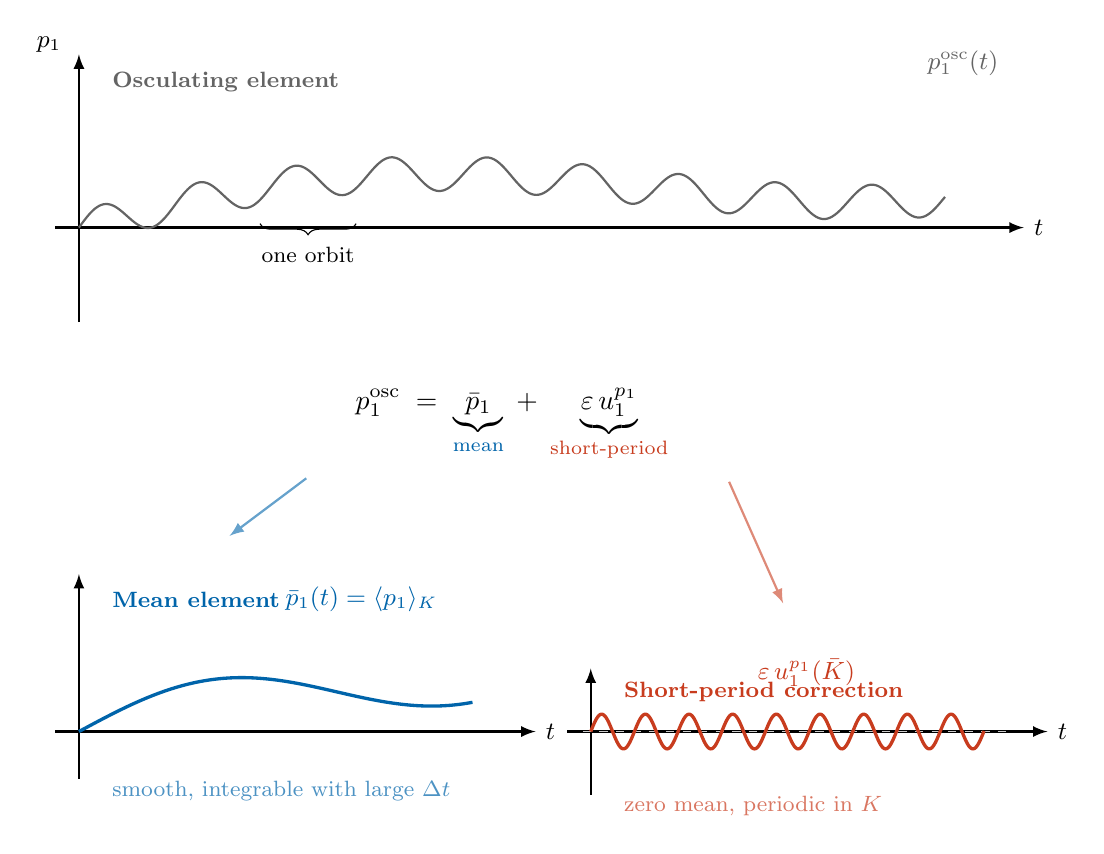
\begin{tikzpicture}[>=latex, font=\small]

% ===================================================================
% Waveforms — domain x in [0, 11] for top panel
%
%   Slow trend:  S(x) = 0.07*x + 0.40*sin(25*x)
%                  drift ~0.77 over full domain; sin with period 14.4
%                  so ~0.76 full cycles -> visible undulation
%                  max arg: 25*11 = 275 (safe)
%   Fast oscill: F(x) = 0.22*sin(295*x)
%                  ~9 fast cycles; max arg: 295*11 = 3245 (safe)
%
% Bottom panels compress [0,11] -> [0,5] via factor 2.2:
%   S_c(x) = 0.154*x + 0.40*sin(55*x)   max arg: 275 (safe)
%   F_c(x) = 0.22*sin(649*x)             max arg: 3245 (safe)
% ===================================================================

% ===== TOP PANEL: Osculating element =====
\begin{scope}[shift={(0,6.2)}]
  \draw[->, thick] (-0.3,0) -- (12,0) node[right] {$t$};
  \draw[->, thick] (0,-1.2) -- (0,2.2);
  \node[anchor=south east] at (-0.1,2.1) {$p_1$};

  \node[anchor=north west, font=\bfseries\footnotesize, orbitgray]
    at (0.3,2.1) {Osculating element};

  % Osculating = slow + fast
  \draw[orbitgray, thick, smooth, samples=550, domain=0:11]
    plot (\x, {0.07*\x + 0.40*sin(25*\x) + 0.22*sin(295*\x)});

  \node[orbitgray, anchor=south east] at (11.8, 1.8) {$p_1^{\mathrm{osc}}(t)$};

  % "one orbit" brace: period = 360/295 ~ 1.22 in x-units
  % At x ~ 2.5, sin(25*2.5)=sin(62.5)~0.89, slow part ~ 0.175+0.356=0.53
  % The curve oscillates between ~0.53-0.22=0.31 and ~0.53+0.22=0.75
  % Place brace just below the trough
  \draw[decorate, decoration={brace, amplitude=4pt, mirror}]
    (2.3, 0.05) -- (3.52, 0.05)
    node[midway, below=5pt, font=\footnotesize] {one orbit};
\end{scope}

% ===== CONNECTING EQUATION =====
\node[fill=white, inner sep=5pt, font=\normalsize] at (5.5, 3.7) {%
  $\displaystyle p_1^{\mathrm{osc}} \;=\;
    \underbrace{\bar{p}_1}_{\text{\color{accent}mean}}
    \;+\;
    \underbrace{\varepsilon\, u_1^{p_1}}_{\text{\color{highlight}short-period}}$};

% Arrows from equation to sub-panels
\draw[->, thick, accent!60, shorten >=4pt, shorten <=4pt]
  (3.0, 3.1) -- (1.8, 2.2);
\draw[->, thick, highlight!60, shorten >=4pt, shorten <=4pt]
  (8.2, 3.1) -- (9.0, 1.3);

% ===== BOTTOM LEFT: Mean element =====
\begin{scope}[shift={(0,-0.2)}]
  \draw[->, thick] (-0.3,0) -- (5.8,0) node[right] {$t$};
  \draw[->, thick] (0,-0.6) -- (0,2.0);

  \node[anchor=north west, font=\bfseries\footnotesize, accent]
    at (0.3,1.9) {Mean element};

  % Slow trend only, compressed domain
  \draw[accent, very thick, smooth, samples=200, domain=0:5]
    plot (\x, {0.154*\x + 0.40*sin(55*\x)});

  \node[accent, anchor=south west] at (2.5, 1.4)
    {$\bar{p}_1(t) = \langle p_1 \rangle_K$};

  \node[accent!70, font=\footnotesize, anchor=north west] at (0.3, -0.5)
    {smooth, integrable with large $\Delta t$};
\end{scope}

% ===== BOTTOM RIGHT: Short-period correction =====
\begin{scope}[shift={(6.5,-0.2)}]
  \draw[->, thick] (-0.3,0) -- (5.8,0) node[right] {$t$};
  \draw[->, thick] (0,-0.8) -- (0,0.8);

  \draw[gray!40, dashed] (-0.1,0) -- (5.3,0);

  \node[anchor=north west, font=\bfseries\footnotesize, highlight]
    at (0.3,0.75) {Short-period correction};

  % Fast oscillation only (zero mean)
  \draw[highlight, very thick, smooth, samples=500, domain=0:5]
    plot (\x, {0.22*sin(649*\x)});

  \node[highlight, anchor=south west] at (2.0, 0.45)
    {$\varepsilon\, u_1^{p_1}(\bar{K})$};

  \node[highlight!70, font=\footnotesize, anchor=north west] at (0.3, -0.7)
    {zero mean, periodic in $K$};
\end{scope}

\end{tikzpicture}
\end{document}
